\begin{frame}
    \frametitle{Why do we need statistics for malware datasets?}
    \centering

    Without the right tools, malware datasets are a stream of bytes

    \begin{figure}[!ht]
        \includegraphics[width=0.75\textwidth]{figures/stase/matrix.jpg}
    \end{figure}

\end{frame}

\subsection[STASE]{STASE:~statistics for malware datasets}

\begin{frame}
    \vfill
    \centering
    \usebeamerfont{title}

    \begin{beamercolorbox}[sep=8pt,center,shadow=true,rounded=true]{title}
        \textbf{STASE}:\\
        statistics for malware datasets

        \small{}

        \bigskip{}

        \textit{
            On the Lack of Consensus in Anti-Virus Decisions:\\
            Metrics and Insights on Building Ground Truths \\
            of Android Malware with VirusTotal
        }
            
        \bigskip{}

        13th Conference on Detection of Intrusions and \\
        Malware \& Vulnerability Assessment (DIMVA)
    \end{beamercolorbox}

    \vfill
\end{frame}


\begin{frame}
    \frametitle{Reminders and methodology}
    \small{}

    \begin{columns}
        \begin{column}{0.8\textwidth}
            \begin{block}{}
                \centering
                \textbf{Reminders}
            \end{block}
            \begin{itemize}
                \item Experts need statistics to understand malware sets
                \begin{itemize}
                    \item e.g., level of diversity, confidence, agreement
                \end{itemize}
                \item Antivirus are an abundant source of information
                \item How to verify the quality of antivirus results?
            \end{itemize}

            \begin{block}{}
                \centering
                \textbf{Methodology}
            \end{block}
            \begin{itemize}
                \item Derive 3 datasets from typical research settings
                \item Compute 8 metrics to quantify their differences
                \item Study the impact on antivirus \textit{decisions} and \textit{labels}
                \begin{itemize}
                    \item where \textit{decisions} = yes/no, \textit{labels} = description
                \end{itemize}
            \end{itemize}
        \end{column}

        \begin{column}{0.3\textwidth}
            \begin{figure}[!ht]
                
\includegraphics[width=0.95\textwidth]{figures/stase/glass.jpg}
            \end{figure}
        \end{column}
    \end{columns}

\end{frame}

\begin{frame}
    \frametitle{Measuring the agreement between antivirus decisions}
    \centering

    \cmark: is a malware, \xmark: not a malware, \openbox{} no decision
    \vspace{-15pt}

    \begin{columns}
        \begin{column}{0.5\textwidth}
            \begin{table}[!ht]
                \resizebox{\textwidth}{!}{
                    \begin{tabular}{c|c c c}
    & AV1 & AV2 & AV3 \\
    \hline
    App 1 & \cmark{} & \cmark{} & \cmark{} \\
    App 2 & & & \\
    App 3 & \xmark{} & \xmark{} & \xmark{} \\
\end{tabular}

                }
                \smallskip{}
                \caption{\footnotesize{\textit{High} level of agreement}}
            \end{table}
        \end{column}

        \begin{column}{0.5\textwidth}
            \begin{table}[!ht]
                \resizebox{\textwidth}{!}{
                    \begin{tabular}{c|c c c}
    & AV1 & AV2 & AV3 \\
    \hline
    App 1 & \cmark{} & \xmark{} & \\
    App 2 & \xmark{} & & \cmark{} \\
    App 3 & & \cmark{} & \xmark{} \\
\end{tabular}

                }
                \smallskip{}
                \caption{\footnotesize{\textit{Low} level of agreement}}
            \end{table}
        \end{column}
    \end{columns}

    \medskip{}

    \begin{table}[!ht]
        \resizebox{0.5\textwidth}{!}{
            \begin{tabular}{c|c c c}
    & AV1 & AV2 & AV3 \\
    \hline
    App 1 & \cmark{} & \cmark{} & \xmark{} \\
    App 2 & \xmark{} & \xmark{} & \xmark{} \\
    App 3 & \cmark{} & \cmark{} & \xmark{} \\
\end{tabular}

        }
        \smallskip{}
        \caption{\footnotesize{\textit{Medium} level of agreement}}
    \end{table}

\end{frame}

\begin{frame}
    \frametitle{Synchronicity: agreement between antivirus detections}
    \vspace{-10pt}

    \footnotesize{
        \begin{gather*}
            Synchronicity(\mathcal{B}) = \frac{\sum^n_{j=1} \sum^{n}_{j'=1}
            \dfrac{|C_j \cap C_{j'}|}{\min(|C_j|,|C_{j'}|)}}{n (n-1)} \\
            \text{ with } j \neq j', C_j \in \mathcal{B}, C_{j'} \in \mathcal{B},
            \text{and } \mathcal{B} \text{ is the matrix of antivirus decisions}
        \end{gather*}
    }

    \vspace{-20pt}

    \begin{columns}
        \begin{column}{0.55\textwidth}
            \vspace{-15pt}
            \centering
            \small{}

            \bigskip{}
            \textbf{Observations}:\\
            \smallskip{}
            \begin{itemize}
                \item Local agreements (red clusters)
                \item Global disagreement (white tone)
            \end{itemize}

            \bigskip{}
            \textbf{Conclusions}:\\
            \smallskip{}
            \begin{itemize}
                \item Lack of consensus in decisions
                \item Antivirus are not interchangeable
            \end{itemize}

        \end{column}

        \begin{column}{0.5\textwidth}
            \begin{figure}[!ht]
                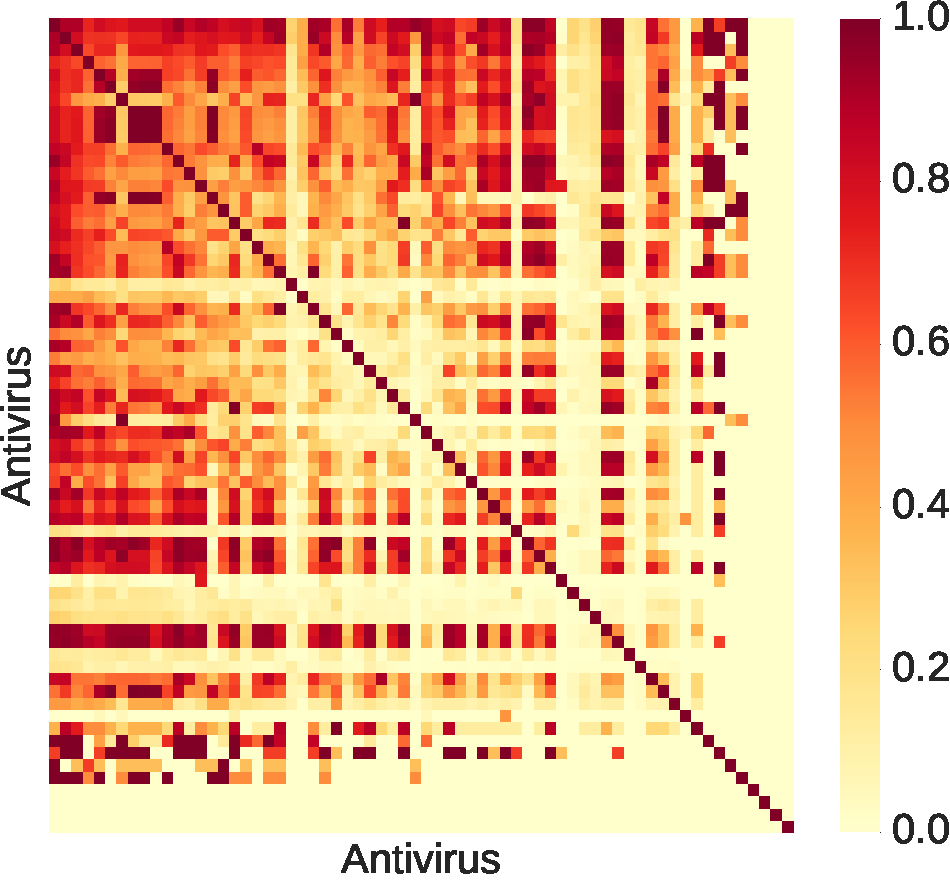
\includegraphics[width=0.95\textwidth]{figures/stase/synchronicity.pdf}
                \caption{\scriptsize{
                    Overlap between antivirus (66$\times$66) \\
                    symmetrical w.r.t.~the diagonal
                }}
            \end{figure}
        \end{column}
    \end{columns}

\end{frame}

\begin{frame}
    \frametitle{Other metrics for analyzing antivirus detections}
    \centering

    \begin{block}{}
        \centering
        Synchronicity \\
    \end{block}
    \small{
        What is the likelihood for any pair of distinct antivirus to agree \\
        on a given malware sample in the resulting ground truth?
    }

    \begin{block}{}
        \centering
        \textbf{Equiponderance} \\
    \end{block}
    \small{
        Is the resulting ground truth dominated by only a few antiviruses, \\
        or do all antivirus contribute the same amount of information?
    }

    \begin{block}{}
        \centering
        \textbf{Exclusivity} \\
    \end{block}
    \small{
        What is the proportion of malware samples that were included \\
        only due to one antivirus engine in the resulting ground truth?
    }

    \begin{block}{}
        \centering
        \textbf{Recognition} \\
    \end{block}
    \small{
        Have malware samples that were included been marginally or \\
        widely recognized to be malicious in the resulting ground truth?
    }

\end{frame}

\begin{frame}
    \frametitle{Measuring the cacophony between antivirus labels}
    \centering

    \bigskip{}

    \begin{columns}
        \begin{column}{0.5\textwidth}
            \begin{table}[!ht]
                \resizebox{0.97\textwidth}{!}{
                    \begin{tabular}{c|c c c}
    & AV1 & AV2 & AV3 \\
    \hline
    App 1 & adrd & adrd & adrd \\
    App 2 & & & \\
    App 3 & adwo & adwo & adwo \\
\end{tabular}

                }
                \smallskip{}
                \caption{\footnotesize{\textit{Low} level of cacophony}}
            \end{table}
        \end{column}

        \begin{column}{0.5\textwidth}
            \begin{table}[!ht]
                \resizebox{\textwidth}{!}{
                    \begin{tabular}{c|c c c}
    & AV1 & AV2 & AV3 \\
    \hline
    App 1 & adrd & adwo & \\
    App 2 & mirai.1 & mirai.a & mirai \\
    App 3 & trojan & spyware & trj \\
\end{tabular}

                }
                \smallskip{}
                \caption{\footnotesize{\textit{High} level of cacophony}}
            \end{table}
        \end{column}
    \end{columns}

    \medskip{}

    \begin{table}[!ht]
        \resizebox{0.5\textwidth}{!}{
            \begin{tabular}{c|c c c}
    & AV1 & AV2 & AV3 \\
    \hline
    App 1 & adrd & adrd & adwo \\
    App 2 & mirai & mirai.1 & mirai.1 \\
    App 3 & trojan & & trojan \\
\end{tabular}

        }
        \smallskip{}
        \caption{\footnotesize{\textit{Medium} level of cacophony}}
    \end{table}

\end{frame}

\begin{frame}
    \frametitle{Divergence: cacophony of antivirus labels per sample}
    \vspace{-10pt}

    \scriptsize{
        \begin{gather*}
            Divergence(\mathcal{L}) = \dfrac{(\sum_{i=1}^m X_i) - n}{positives(\mathcal{L}) - n}
            \text{ with } X_i = \{distincts(R_i) : R_i \in \mathcal{L}, 1 \leq i \leq m\}, \\
            \mathcal{L} \text{ is the matrix of antivirus labels},
            \text{ and } n \text{ is the total number of antivirus}
        \end{gather*}
    }

    \vspace{-20pt}

    \begin{columns}
        \begin{column}{0.5\textwidth}
            \begin{figure}[!ht]
                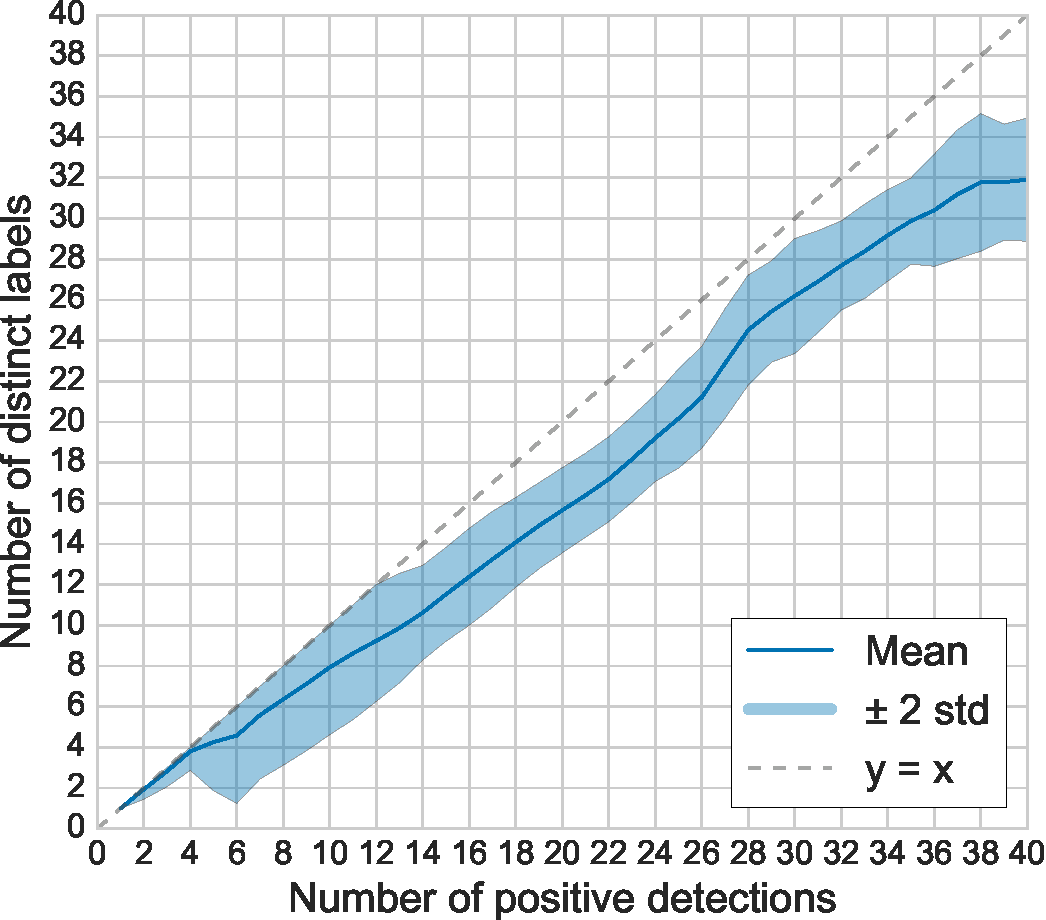
\includegraphics[width=\textwidth]{figures/stase/divergence.pdf}
                \caption{\footnotesize{Relation between distinct labels and positive detections per sample}}
            \end{figure}
        \end{column}

        \begin{column}{0.55\textwidth}
            \vspace{-15pt}
            \centering
            \small{}

            \bigskip{}
            \textbf{Observations}:\\
            \smallskip{}
            \begin{itemize}
                \item Strong linear relation (y = x)
                \item Not the ideal scenario (y $\simeq$ 1)
            \end{itemize}

            \bigskip{}
            \textbf{Conclusions}:\\
            \smallskip{}
            \begin{itemize}
                \item More decisions, more labels
                \item Cacophony between antivirus
            \end{itemize}

        \end{column}
    \end{columns}

\end{frame}

\begin{frame}
    \frametitle{Other metrics for analyzing antivirus labels}
    \centering

    \begin{block}{}
        \centering
        Divergence \\
    \end{block}
    \small{
        To what extent do antivirus provide an inconsistent label regarding other antivirus for each sample in the resulting ground truth?
    }

    \begin{block}{}
        \centering
        \textbf{Uniformity} \\
    \end{block}
    \small{
        Are the labels associated with malware samples evenly distributed \\
        or converging to a single label in the resulting ground truth?
    }

    \begin{block}{}
        \centering
        \textbf{Genericity} \\
    \end{block}
    \small{
        What is, on average for an antivirus, the degree of reuse of a label to \\
        characterize several malware samples in the resulting ground truth?
    }

    \begin{block}{}
        \centering
        \textbf{Consensuality} \\
    \end{block}
    \small{
        To what extent can we rely on the most frequent label
        as an authoritative label for each sample in the resulting ground truth?
    }

\end{frame}


\begin{frame}
    \frametitle{Datasets and results observed for Android malware}
    \centering

    \begin{block}{}
        \centering
        \textbf{Datasets}
    \end{block}
    \vspace{-11pt}
    \begin{table}[!ht]
        \resizebox{\textwidth}{!}{
            \begin{tabular}{|c|c|c|c|c|}
    \hline
    & Initial Dataset & Baseline dataset &  Genome dataset & Filtered dataset \\ \hline
    Notation & $\mathcal{D}_{initial}$& $\mathcal{D}_{baseline}$& $\mathcal{D}_{genome} $& $\mathcal{D}_{filtered}$\\% \hline
    Applications & 2\,117\,825 & 689\,209 & 1\,248 & 44\,615 \\% \hline
    \textbf{Antivirus} & 66 & 66 & 66 & 10 \\% \hline
    \textbf{Discard adware} & No & No & No & Yes \\% \hline
    \textbf{Analyzed manually} & No & No & Yes & No \\% \hline
    \textbf{Detection threshold} & $\geq 0$& $\geq 1$& $\geq 0$& $\geq 2$ \\
    \hline
\end{tabular}

        }
        \caption{\footnotesize{Experimental ground truth settings (in bold) studied with our metrics}}
    \end{table}

    \vspace{-10pt}

    \begin{block}{}
        \centering
        \textbf{Results}
    \end{block}

    STASE can highlight the differences between malware datasets

    \begin{table}[!ht]
        \resizebox{\textwidth}{!}{
            \begin{tabular}{|c|c|c|c|c||c|c|c|c|c|}
    \hline
    & Equip. & Exclu. & Recog. & \textbf{Synchronicity} & \textbf{Divergence} & Unifo. & Gener.  & Conse. \\
    \hline
    $\mathcal{D}_{baseline}$ & 0.27 & 0.31 & 0.09 & \textbf{0.32} & \textbf{0.77}& 0.001 & 0.97  & 0.21 \\
    $\mathcal{D}_{genome}$ & 0.48 & 0 & 0.48 & \textbf{0.41} & \textbf{0.87} & 0.04 & 0.82  & 0.06 \\
    $\mathcal{D}_{filtered}$ & 0.59 & 0 & 0.36 & \textbf{0.75} & \textbf{0.95} & 0.01 & 0.87 & 0.05 \\
    \hline
\end{tabular}

        }
        \caption{\footnotesize{Summary of STASE metrics for three ground truth construction settings}}
    \end{table}

    % \begin{itemize}
    %     \item We observe higher values of \emph{Recognition} and \emph{Synchronicity} metrics for $\mathcal{D}_{genome}$ and $\mathcal{D}_{filtered}$ compare to $\mathcal{D}_{base}$ dataset
    %     \begin{itemize}
    %         \item this observation suggests that these datasets were built with samples that are well known to be malicious in the industry
    %     \end{itemize}

    %     \smallskip{}

    %     \item The value of \emph{Genericity} is higher and the \emph{Equiponderance} is lower in $\mathcal{D}_{base}$ compared to $\mathcal{D}_{genome}$ and $\mathcal{D}_{filtered}$ dataset
    %     \begin{itemize}
    %         \item this indicates that antivirus detections are less generic and more balanced across antivirus in the former datasets
    %     \end{itemize}

    %     \smallskip{}

    %     \item The \emph{Divergence} metric is lower and \emph{Consensuality} metric is higher in $\mathcal{D}_{base}$  compared to $\mathcal{D}_{genome}$ and $\mathcal{D}_{filtered}$ datasets
    %     \begin{itemize}
    %         \item the constraints put on building the former datasets has diminished the general agreement between antivirus
    %     \end{itemize}
    % \end{itemize}

\end{frame}

\begin{frame}
    \frametitle{Contributions and conclusions}
    \centering

    \begin{block}{}
        \centering
        \textbf{Contributions}
    \end{block}
    \begin{itemize}
        \item Verify the quality of antivirus results
        \item Study the impacts of ground truth settings
        \item View the properties of malware ground truths
    \end{itemize}

    \medskip{}

    \begin{block}{}
        \centering
        \textbf{Conclusions}
    \end{block}
    \begin{itemize}
        \item Antivirus labels provide valuable descriptions of malware
        \item But there is a lack of agreement between antivirus labels
        \begin{itemize}
            \item e.g., high value of divergence, low level of consensuality
        \end{itemize}
    \end{itemize}

    \medskip{}

    \textbf{How can we retrieve information contained in labels?}

\end{frame}

\begin{frame}
    \frametitle{How to improve the security of Android}

    \begin{tabularx}{\textwidth}{l r}
        \multicolumn{2}{c}{\textbf{Challenge 1:~Definition of Android malware}\vspace{5pt}} \\
        \textbullet~Verify the quality of antivirus results & \textcolor{RED}{STASE} \\
        \dotline{270pt} & \\
        \dotline{270pt} & \\
        \\
        \multicolumn{2}{c}{\textbf{Challenge 2:~Detection of Android malware}\vspace{5pt}} \\
        \textbullet~Study the impacts of ground truth settings & \textcolor{RED}{STASE} \\
        \dotline{270pt} & \\
        \dotline{270pt} & \\
        \\
        \multicolumn{2}{c}{\textbf{Challenge 3:~Comprehension of Android malware}\vspace{5pt}} \\
        \textbullet~View the properties of malware ground truths & \textcolor{RED}{STASE} \\
        \dotline{270pt} & \\
        \dotline{270pt} & \\
    \end{tabularx}

\end{frame}
